% Activate the following line by filling in the right side. If for example the name of the root file is Main.tex, write
% "...root = Main.tex" if the chapter file is in the same directory, and "...root = ../Main.tex" if the chapter is in a subdirectory.

%!TEX root =  ../../../Tesis.tex

\chapter*{Evolution of residues from the cytochrome c oxidase complex engaged in intermolecular contacts}
H�ctor Valverde\footnotemark[1], Manuel Ru�z-Camacho\footnotemark[2], Ian Morilla\footnotemark[1], Francisco Demetrio L�pez\footnotemark[2], Juan Carlos Aledo\footnotemark[1]$^,$\footnotemark[3]

\footnotetext[1]{Departamento de Biolog�a Molecular y Bioqu�mica. Facultad de Ciencias. Universidad de M�laga, 29071 M�laga, Spain}
\footnotetext[2]{Departamento de Estad�stica e Investigaci�n Operativa. Facultad de Ciencias. Universidad de M�laga, 29071 M�laga, Spain}
\footnotetext[3]{Corresponding author: caledo@uma.es}

\emph{Keywords: Coevolution, COX, evolvability, mtDNA, natural selection, protein evolution, protein-protein interaction.}

\section*{Abstract}
Respiratory complexes are encoded by two genomes (mtDNA and nDNA). Although the importance of intergenomic coadaptation is acknowledged, the forces and constrains shaping such coevolution are largely unknown. Previous works using cytochrome c oxidase (COX) as a model enzyme, have led to the so-called ``optimizing interaction'' hypothesis. According to this view, mtDNA-encoded residues close to nDNA-encoded residues evolve faster than the rest of positions, favouring the optimization of protein-protein interfaces. Herein, using evolutionary data in combination with structural information of COX, we show that failing to discern the effects of interaction from other structural effects, can lead to deceptive conclusions such as the ``optimizing hypothesis''. Once spurious factors have been accounted for, data analysis shows that mtDNA-encoded residues engaged in contacts are, in general, more constrained than their noncontact counterpart. Nevertheless, noncontact residues from the surface of COX 1 subunit are a remarkable exception, being subjected to an exceptionally high purifying selection. We also report that mtDNA-encoded residues involved in contacts with other mtDNA-encoded subunits, are more constrained than mtDNA-encoded residues interacting with nDNA-encoded polypeptides. This differential behaviour cannot be explained on the basis of thermodynamic stability, since interactions between mtDNA-encoded subunits contribute more weakly to the complex stability than those interactions between subunits encoded by different genomes. Finally, among nDNA-encoded subunits, contact residues are more conserved than noncontact residues, being COX 5A an exception.

\section*{Introduction}
Although mitochondria are involved in many aspects of cell function, including proliferation (Aledo 2004), apoptosis (Suen et al. 2008) and aging (Aledo et al. 2010), their central role is related to energy transduction in oxidative phosphorylation (OXPHOS). The mitochondrial proteins responsible for the OXPHOS are encoded by two genomes. In mammals, the mitochondrial genome (mtDNA) encodes for 13 polypeptides that interact with a large number of nuclear-encoded (nDNA-encoded) polypeptides to form the functional complexes I, III, IV and V of the OXPHOS system. Given that each mtDNA gene product must interact with proteins encoded by the nuclear genome to carry out its functions, coevolution between mtDNA and nDNA leading to intergenomic coadaptation is expected.

As a consequence of their critical function, mutations altering the structure of these oligomeric complexes must face the close scrutiny of natural selection. In this way, natural selection will favour evolutionary coadaptation of interacting proteins, either to improve physiological functions (Schmidt et al. 2005), or just to maintain the fitness through compensatory changes after a slightly deleterious mutation has been fixed by genetic drift (Osada and Akashi 2011). Whatever the driving force may be, there are numerous examples of the biological importance of intergenomic coadaptation. In this sense, xenomitochondrial cybrid cells constructed using nDNA from one species and mtDNA from a close species were viable and had a functional OXPHOS, whereas more divergent species failed to produce functional OXPHOS complexes (Kenyon and Moraes 1997; Barrientos et al. 2000; McKenzie 2003). These results underline the importance of cytonuclear coevolution. Similar conclusions were derived from studies where repeated backcrossing of genetically isolated populations of the copepod \textit{Tigriopus californicus}, allowed to place the maternally inherited mtDNA genome of one population with the paternal nDNA of another. These interpopulation hibrids exhibited a defective OXPHOS system (Edmands and Burton 1999). A third line of evidence suggesting that OXPHOS proteins have coevolved to function optimally, comes from epistatic studies where mutations in mtDNA genes that are pathogenic in humans have been observed in naturally occurring genomes from nonhuman mammals (de Magalh�es 2005; Azevedo et al. 2009).

While the above studies emphasize the relevance of coevolution between interacting proteins, they do not provide much insight on the forces and constrains shaping such coevolution. In an attempt to explore the evolutionary dynamics of these protein-protein interactions, Schmidt and co-workers used cytochrome c oxidase (COX) as a model of OXPHOS holoenzyme. These authors analysed the rate of nonsynonymous substitutions within a set formed by mtDNA-encoded residues in physical proximity to nDNA-encoded amino acids, and compared it with that computed for the rest of mtDNA-encoded residues, which are not in contact with nDNA-encoded polypeptide chains. They concluded that mtDNA-encoded residues in close contact with amino acids being encoded by the nucleus, evolve faster than the rest of mtDNA-encoded residues (Schmidt et al. 2001). This result was interpreted as being due to many different amino acid replacements among the close contact residues being required to optimize this protein's interaction with other proteins. Actually, the authors referred to such a state as an ``optimizing interaction''. In contrast, when COX residues encoded by nDNA were segregated on the basis of proximity to mtDNA-encoded residues, and the rates of nonsynonymous substitution were analysed, the conclusion reached was the opposite. That is, those nDNA-encoded residues in contact with mtDNA-encoded amino acids, evolve more slowly than the rest of nDNA-encoded residues (Schmidt et al. 2001).

These striking results have been often cited as an example of the differential forces driving mtDNA and nDNA evolution (Willett 2003; Das et al. 2004; Castellana et al. 2011). While the constrained evolution of nDNA-encoded interacting residues is in line with the prevailing view that protein evolution is generally conservative and constraining interactions are typical, the observation that mtDNA-encoded interacting residues evolve at much higher rates than non interacting amino acids, if confirmed as a bona fide observation, deserved a sound explanation. Herein, we have revisited the ``optimizing interaction'' hypothesis. Using a comprehensive number of mammalian taxa and extended statistic analyses (Fig. \ref{paper31}), we have found that interacting mtDNA-encoded residues, alike interacting nDNA-encoded residues, are subjected to higher constraints than their corresponding non-interacting counterparts. We also provide the keys to understand why previous studies failed to reach similar conclusions. In addition, we show an intriguing difference in the evolutionary rate of mtDNA-encoded residues depending on whether they contact with nDNA-encoded subunits or with other mtDNA- encoded subunits.

% Fig 1
\begin{figure}
\centering
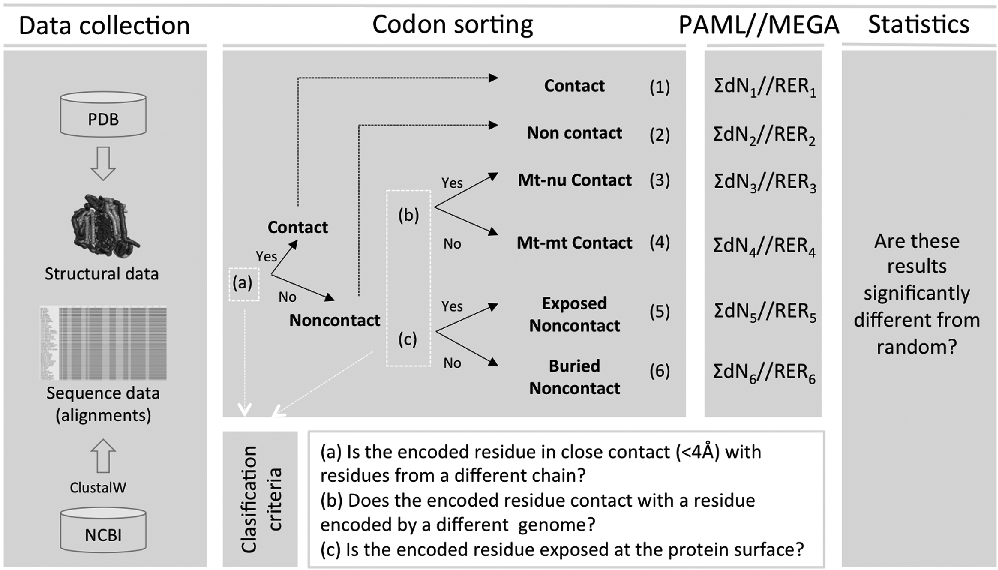
\includegraphics[width=0.8\textwidth]{Apendices/Publicaciones/Contact/Figures/figure1.pdf}
\caption{\small{Flowchart for the main methodological procedure adopted. Once sequence and structural data were collected, aligned codons were sorted into different subsets according to the criteria sketched in the figure (details are given in the text). Afterwards, pairwise nonsynonyomous sequence divergences were calculated for each subset using PAML. The sum for all comparisons yields ${\Sigma}dN_i$, where the subscript i denotes the subset. In addition, the mean relative evolutionary rate (RER) for each subset was computed using MEGA5. Finally, to assess whether the values of these variables were significantly different between subsets, suitable statistical tests, which are described through the text, were carried out.}}
\label{paper31}
\end{figure}
%

\section*{Results and discussion}
\subsection*{Discerning the effects of residue interaction on the evolutionary rate from other structural effects.}
The optimizing interaction hypothesis arose from the observation that mtDNA-encoded residues from COX in close contact with nDNA-encoded amino acids, showed a higher rate of nonsynonymous substitutions than the rest of mtDNA-encoded residues (Schmidt et al. 2001). Since these rates of nonsynonymous substitutions were originally calculated using orthologous sequences from only 26 mammalian species, we wanted to start by re-assessing this issue using a more comprehensive collection of sequences from 371 mammalian taxa. In this way, using our extensive alignment and the methodology described by Schmidt et al., the set formed by the aligned codons from the three mtDNA-encoded COX subunits (ABC), was split into two subsets: ABC$_{Mt-nu\_Contact}$ and its complement, (ABC$_{Mt-nu\_Contact}$)$^c$. The former encompassed those triplets encoding for residues close to nDNA-encoded aminoacids in the holoenzyme, while the latter set contained all the codons from chain A, B and C, which encoded amino acids that are not in contact with nDNA-encoded residues (Fig. \ref{paper32}). The calculated interaction ratio, R$_{ABC_{Mt-nu\_Contact},(ABC_{Mt-nu\_Contact})^c}$, was 1.805 $\pm$ 10$^{-4}$, significantly greater than 1. Although this result is in line with the data reported by Schmidt and coworkers, such an observation by itself is, in our opinion, insufficient to support the conclusion that contact residues are subjected to a positive selection, as suggested in previous works (Schmidt et al. 2001).

% Fig 2
\begin{figure}
\centering
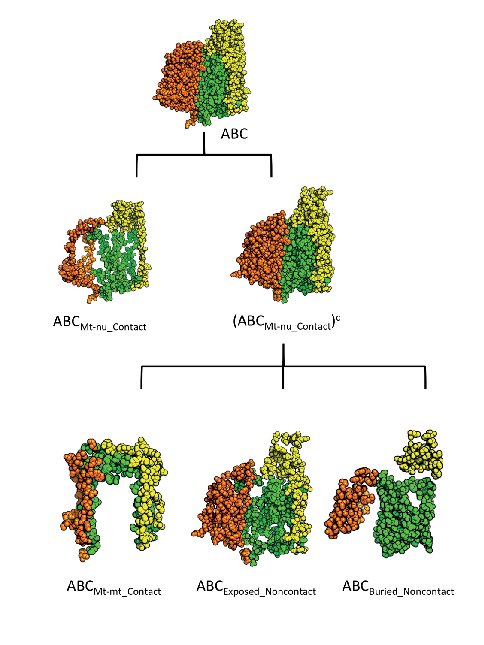
\includegraphics[width=0.7\textwidth]{Apendices/Publicaciones/Contact/Figures/figure2.pdf}
\caption{\small{Structural view of mitochondrially encoded COX residues. COX core, consisting of COX subunits 1 (chain A in green), 2 (chain B in yellow) and 3 (chain C in orange) is shown on the top of the figure. The spatial distribution of those residues in close contact with nDNA-encoded subunits (ABC$_{Mt\_nu\_Contact}$) is also shown. The set formed by mtDNA-encoded residues that are not in contact with nDNA-encoded subunits, (ABC$_{Mt\_nu\_Contact}$)$^c$, was partitioned into three disjoint subsets: ABC$_{Mt\_mt\_Contact}$, which is formed by those residues contacting only with other mtDNA-encoded residues; ABC$_{Exposed\_Noncontact}$, encompassing residues accessible to the solvent that are not involved in intersubunit contacts; and ABC$_{Buried\_Noncontact}$, which contains all those residues that being buried inside the protein are not available for interusubunit contacts. The spatial distributions of the residues belonging to each of these subsets are shown at the bottom of the figure.}}
\label{paper32}
\end{figure}
%

In this sense, a number of considerations need to be addressed before any conclusion can be reached. For instance, the set formed by mtDNA-encoded residues that are not in contact with nDNA-encoded amino acids, used as reference to compute the interaction ratio, represents a heterogeneous collection of residues. Thus, while the amino acids belonging to the ABC$_{Mt-nu\_Contact}$ group are mainly located at the protein surface, a significant part of the noncontact residues are buried into the protein structure (Fig. \ref{paper32}). This observation is relevant because we have recently reported that, for mtDNA-encoded proteins, alike proteins from other genetic origins, buried residues are most likely to remain conserved during evolution compared to their solvent exposed counterparts (Aledo et al. 2012). Therefore, if we want to address the effects of residue interaction on the evolutionary rate, and discern them from other structural effects such as the solvent exposure, the noncontact set used as reference should be restricted to avoid buried residues.

Although the above mentioned restriction is necessary, yet it is not sufficient to build a
suitable reference set. Indeed, the resulting set of such a restriction still contains a group of
residues that may bias the results and mislead the conclusions. We are referring to the
collection formed by those amino acids implicated in protein-protein interactions involving
only contacts between mtDNA-encoded residues (see ABC$_{Mt-mt\_Contact}$ in Figure \ref{paper32}). Since the
evolvability of this category of residues has not been previously characterized, we excluded
them from the reference set, which finally was formed only by those mtDNA-encoded residues exposed at the protein surface that are not involved in any sort of intersubunit contacts. This reference set is referred to as ABC$_{Exposed\_Noncontact}$ (Fig. \ref{paper32}).

Once the partition of the initial data set had been carried out as described above and
illustrated in Figure \ref{paper32}, we next computed diverse evolutionary variables to characterize the
relative evolvability of the following three sets: ABC$_{Mt-nu\_Contact}$, ABC$_{Mt-mt\_Contact}$ and
ABC$_{Exposed\_Noncontact}$, all of them containing only codons for amino acids exposed at the protein surface. The results of such analyses are described next.

\subsection*{Differential behaviour between Mt-mt and Mt-nu interactions.}

To assess the relative evolvability of each category of residue we used different approaches. One of these, consisted in calculating the so-called relative evolutionary rate (RER). Briefly, for each mtDNA-encoded subunit, the RER of each position was computed using MEGA 5 (Tamura et al. 2011), which implements a maximum likelihood method to model evolutionary rate differences among sites. These rates were scaled such that the average evolutionary rate across all sites is 1. In this way, sites showing a rate lower than 1 are evolving slower than average, while those with a rate higher than 1 are evolving faster than average. As it can be observed in Table \ref{TableSigmadN}, among all exposed residues, those involved in interactions between different mtDNA-encoded chains were the most constrained, showing RER values well below the unit, regardless the mtDNA-encoded subunit being considered (Table \ref{TableSigmadN}). This observation indicates a much stronger purifying selection among Mt-mt Contact residues than among Mt-nu Contact amino acids. To substantiate this conclusion, a different approach was followed. For each of the three subsets of exposed residues (Exposed Noncontact, Mt-nu Contact and Mt-mt Contact) as well as for the Buried Noncontact subset, the number of nonsynonymous substitutions per nonsynonymous site, dN, was calculated from pairwise comparisons. The sum of these nonsynonymous sequence divergences for all the pairwise comparisons was computed and denoted as ${\Sigma}dN$. In line with the results based on RER, the Mt-mt Contact set exhibited the lower ${\Sigma}dN$ values among all the exposed residues (Table \ref{TableSigmadN}). Since dN is informative of the combined effect of mutation and selection, we used ${\Sigma}dN$ as a proxy of the evolvability of the corresponding subset of residues being analysed. However, ${\Sigma}dN$ averages over all the analysed mammalian species and, therefore, it provides little information on whether the evolutionary dynamics described above, has a broad phylogenetic distribution and is present in most mammalian lineages. To address this issue, phylogenetic trees were used to apportion the nonsynonymous substitutions for the different residue subsets. As it can be deduced from Fig. \ref{paper33}, all lineages without exception showed much higher dN when the analysed subset was mtDNA-encoded residues contacting with nDNA-encoded subunits, with respect to those contacting with other mtDNA-encoded polypeptides. In most cases, the difference in the dN values computed for these two groups of residues was of one order of magnitude. (See also Supplementary Material-1). All together, these results suggest that those mtDNA-encoded residues in contact with mtDNA-encoded residues from a different chain, are subjected to stronger constrains than those involved in interactions with nDNA-encoded subunits. In addition, this behaviour seems to have a broad phylogenetic distribution and is valid for most mammalian lineages (Fig. \ref{paper33}). To the best of our knowledge, this is the first quantitative study supporting such a conclusion, which may be rationalized as follows. In mammals, the three mtDNA-encoded subunits form the catalytic core of the enzyme, while the 10 nDNA-encoded subunits act as a regulatory shield surrounding the core (Soto et al. 2012). Prokaryote forms of COX boil down to the catalytic core, which seems to have an ancient origin (Castresana et al. 1994). In contrast, eukaryotes possess nuclear genes for additional subunits, the number of which generally increases with the organismal complexity. Although, neither the origin nor the specific function of these additional non-catalytic subunits is completely understood, there is little doubt that they are significantly younger than the proteins conforming the catalytic core (Castresana et al. 1994; Das et al. 2004; Little et al. 2010). On the other hand, it is well known that young proteins tend to experience weaker purifying selection and evolve more quickly than old proteins (Alba and Catresana 2005; Vishnoi et al. 2010). Herein, we propose that what is true for proteins may also be true for interactions. In other words, it is reasonable to assume that within a given protein with a fixed antiquity, those residues involved in ``old interactions'' evolve more slowly than those other residues implicated in ``young interactions''. Describing how selection pressure acts at the interfaces of protein-protein complexes is a fundamental issue with high interest for the structural prediction of macromolecular assemblies. Therefore, although it is out of the scope of the current research, in the future it would be interesting to assess whether the relationship between the strength of selection and the age of the interaction, described herein for mtDNA-encoded COX subunits, also applies to other proteins. To encourage this task, we have released the program that implement part of the workflow sketched in Fig. \ref{paper31}. This program has been submitted into the public repository CPAN under an open source license, which allows any other researcher to modify the software in order to include other structural, evolutionary and statistical analyses that may help to gain insights into the molecular evolution of any particular protein complex of interest. Documentation and guides for users and developers are available at the program website \url{http//mecom.hval.es}.

% Tabla SigmadN
\begin{table}
\centering
\begin{threeparttable}
	\caption{\label{TableSigmadN} \small{Contact residues from mtDNA-encoded subunits evolve differentially depending on the genetic origin of the contacted residue.}}
	\begin{tabular}{c c c c c}
	& \multicolumn{4}{ c }{\textbf{${\Sigma}d_N$}}\\
	\cmidrule[1pt]{2-5}
	& \bf{ABC}
	& \bf{A}
	& \bf{B}
	& \bf{C}
	\\
	\midrule
	\textbf{Exposed\ Noncontact}
	& 5954 $\pm$ 10
	& 2901 $\pm$ 9
	& 10605 $\pm$ 104
	& 8404 $\pm$ 50\vspace{0.3cm}
	\\
	\textbf{(Mt-mt) Contact}
	& 2508 $\pm$ 7
	& 939 $\pm$ 5
	& 3034 $\pm$ 27
	& 5820 $\pm$ 83\vspace{0.3cm}
	\\
	\textbf{(Mt-nu) Contact}
	& 7050 $\pm$ 15
	& 7603 $\pm$ 40
	& 7129 $\pm$ 56
	& 6450 $\pm$ 44\vspace{0.3cm}
	\\
	\textbf{Buried Noncontact}
	& 1968 $\pm$ 3
	& 1252 $\pm$ 4
	& 5586 $\pm$ 70
	& 1230 $\pm$ 14
	\\
	\bottomrule
	\end{tabular}
	
	\begin{tabular}{c c c c c}
	& \multicolumn{4}{ c }{\textbf{\textit{RER}}}\\
	\cmidrule[1pt]{2-5}
	& \bf{ABC}
	& \bf{A}
	& \bf{B}
	& \bf{C}
	\\
	\midrule
	\textbf{Exposed\ Noncontact}
	& 1.27 $\pm$ 2.26
	& 1.03 $\pm$ 2.17
	& 1.52 $\pm$ 1.87
	& 1.48 $\pm$ 2.54\vspace{0.3cm}
	\\
	\textbf{(Mt-mt)\ Contact}
	& 0.41 $\pm$ 0.92
	& 0.26 $\pm$ 0.31
	& 0.32 $\pm$ 0.45
	& 0.88 $\pm$ 1.82\vspace{0.3cm}
	\\
	\textbf{(Mt-nu)\ Contact}
	& 1.60 $\pm$ 2.33
	& 2.33 $\pm$ 2.98
	& 1.21 $\pm$ 1.67
	& 0.90 $\pm$ 1.26\vspace{0.3cm}
	\\
	\textbf{Buried\ Noncontact}
	& 0.41 $\pm$ 0.62
	& 0.39 $\pm$ 0.53
	& 0.78 $\pm$ 1.00
	& 0.16 $\pm$ 0.22
	\\
	\bottomrule
	\end{tabular}
	\begin{tablenotes}
\item{\small{In the upper table, the rates of nonsynonymous substitution per nonsynonymous site, dN, were calculated from pairwise comparisons using the alignment data subsets indicated. The sum of these nonsynonymous sequence divergences for all the pairwise comparisons was computed and denoted as ${\Sigma}dN$. Data are expressed as mean $\pm$ standard deviation. In the lower table, a different approach was used to assess the relative evolvability of the different residue subsets. The relative evolutionary rate of each residue was computed using MEGA 5. These rates were scaled such that the average evolutionary rate across all sites is 1. This means that sites showing a rate lower than 1 are evolving slower than average, and those with a rate higher than 1 are evolving faster than average. A short movie showing multiple views of the protein surface formed by residues engaged in Mt-nu (magenta) and Mt-mt contacts (blue), as well as the surface of those residues that are not involved at all in intersubunit contacts (green), can be seen in Supplementary Material-5.}}% Pie de tabla
\end{tablenotes}
\end{threeparttable}
\end{table}
% Fin de tabla sigmadN

% Fig 3
\begin{figure}
\centering
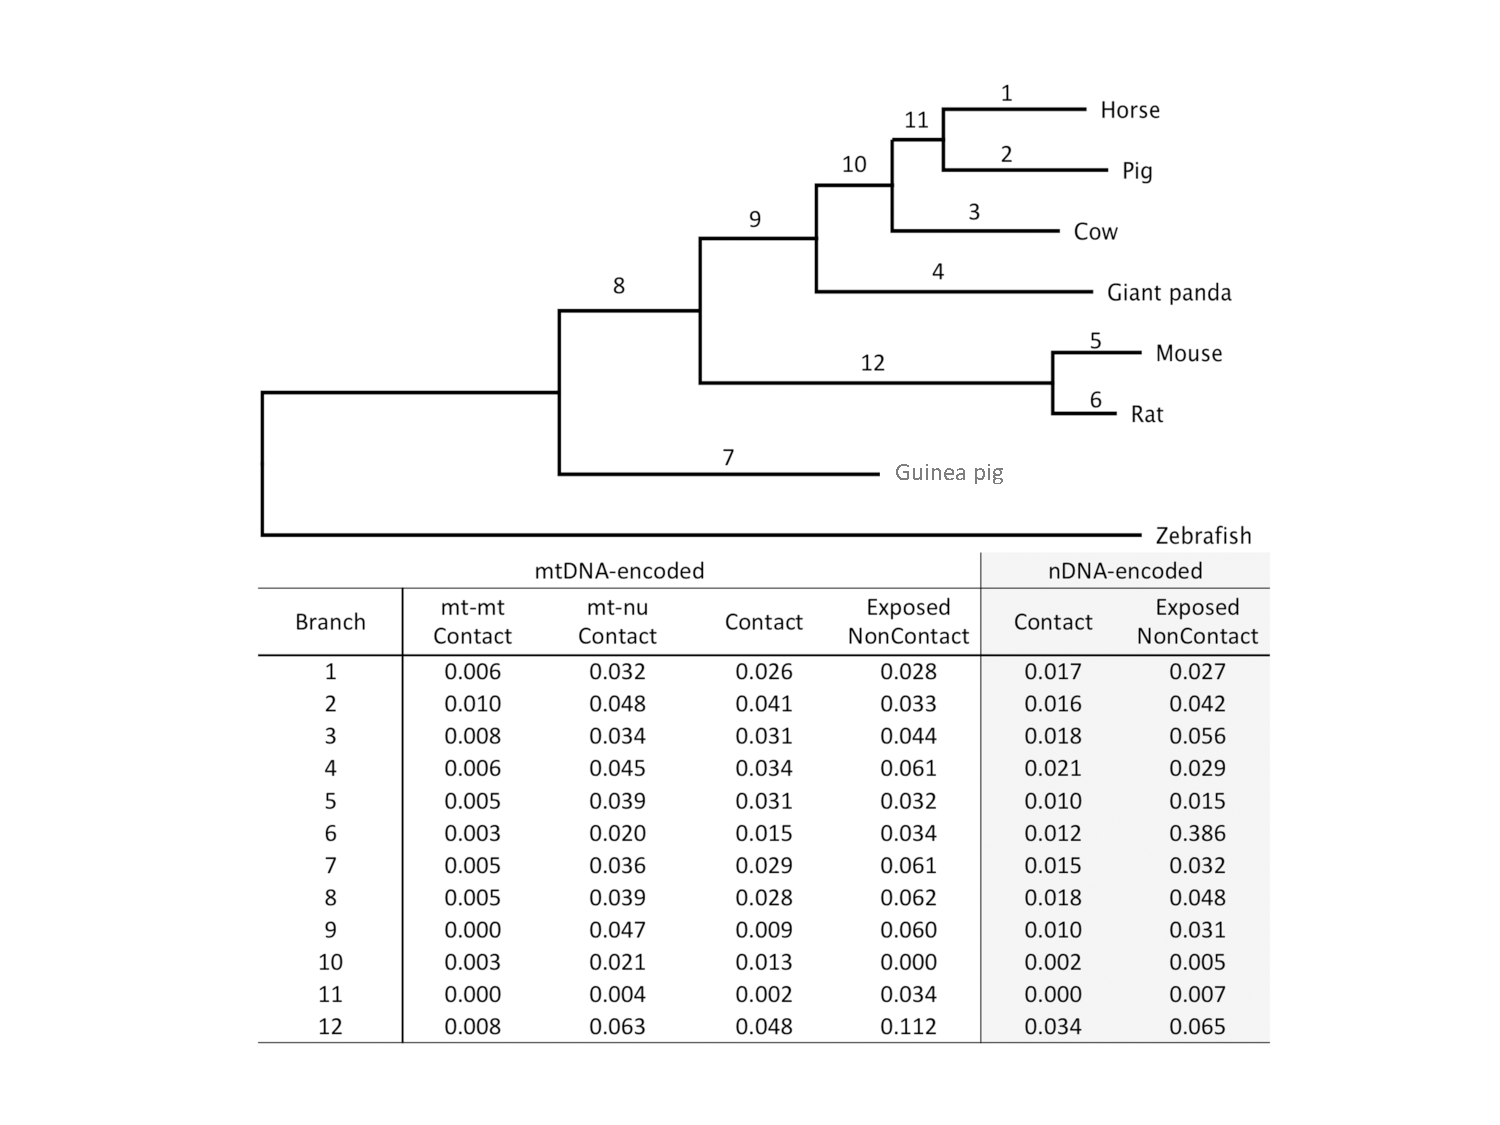
\includegraphics[width=1\textwidth]{Apendices/Publicaciones/Contact/Figures/figure3.pdf}
\caption{\small{Patterns of nonsynonymous substitutions in COX subunits across different mammalian lineages. The phylogenetic tree of seven mammalian species (\textit{Bos taurus}, \textit{Sus scrofa}, \textit{Equus caballus}, \textit{Ailuropoda melanoleuca}, \textit{Mus musculus}, \textit{Rattus norvegicus} and \textit{Cavia porcellus}) for which the gene sequences of the 13 COX subunits were available, was reconstructed using \textit{Arbacia lixula} as an outgroup. The number of nonsynonimous substitutions per nonsynonymous site for each branch is shown for the indicated residue subset.}}
\label{paper33}
\end{figure}
%

\subsection*{Thermodynamic stability does not account for the differential behaviour between Mt-mt and Mt-nu interactions.}

Once we had established that residues from the Mt-mt Contact group are much more constrained than those belonging to the Mt-nu Contact set, we wondered if such differential pattern might have arisen from a differential contribution of these two categories of contacts to the stability of the complex. To address this issue, we carried out an \emph{in silico} alanine scanning mutagenesis. The results of such analysis are summarized in Table \ref{Table3.2}. As expected, changes affecting noncontact residues were among the least destabilizing mutations. On the other hand, from a thermodynamic point of view, residues from the Mt-nu Contact class were much less tolerant to changes than any other kind of residue, including those from the Mt-mt Contact set, which exhibited an intermediate behaviour. Since mutations between residues from the Mt-mt Contact class tend to be less destabilizing than those affecting residues from the Mt-nu Contact group, the higher degree of conservation observed between Mt-mt Contact residues, does not seem to be based on thermodynamic stability, suggesting that functional aspects may be behind the high degree of conservation observed among Mt-mt contact residues.

% Tabla 2
\begin{table}[!hbt]
\centering
\begin{threeparttable}
	\caption{\label{Table3.2} \small{Thermodynamic stability changes.}}
	\begin{tabular}{c c c c c}
	\cmidrule[1pt]{2-5}
	\bf{}
	& \multicolumn{4}{ c }{\bf{$\Delta\Delta$G (kJ/mol)}}\\
	\cmidrule[1pt]{2-5}
	\bf{} 
	& \bf{ABC}
	& \bf{A}
	& \bf{B}
	& \bf{C}
	\\
	\midrule
	\multirow{2}{*}{\bf{Exposed\ Noncontact}}
	& 1.41 $\pm$ 1.51 
	& 1.64 $\pm$ 1.69 
	& 1.20 $\pm$ 1.09 
	& 1.16 $\pm$ 1.38
	\\
	& (\textbf{\textdagger},\textbf{\S\S})
	& (\textbf{\textdagger})
	& (\textbf{\textdagger},\textbf{\S\S})
	& (\textbf{\S}) \vspace{0.3cm}
	\\
	\multirow{2}{*}{\bf{(Mt-mt)\ Contact}}
	& 1.78 $\pm$ 1.97
	& 1.98 $\pm$ 1.65
	& 1.92 $\pm$ 2.61
	& 1.06 $\pm$ 1.52\vspace{0.3cm}
	\\
	& (\textbf{*})
	&
	& 
	& (\textbf{\S}) \vspace{0.3cm}
	\\
	\multirow{2}{*}{\bf{(Mt-nu)\ Contact}}
	& 1.92 $\pm$ 1.60
	& 2.03 $\pm$ 1.55
	& 1.99 $\pm$ 1.47
	& 1.69 $\pm$ 1.73
	\\
	\bf{}
	& (\textbf{**})
	& (\textbf{*})
	& (\textbf{**})
	& (\textbf{*},\bf{\textdagger}) \vspace{0.3cm}
	\\
	\bottomrule
	\end{tabular}
	\begin{tablenotes}
\item{\small{The number of exposed noncontact residues from COX 1-3 were 144, 56 and 92, respectively. The number of mt-mt contact residues from COX 1-3 were 95, 54 and 37, respectively. The number of mt-nu contact residues from chain COX 1-3 were 120, 74 and 82, respectively. Data are expressed as mean $\pm$ standard error.}}
\item{\small{* Significantly different from Exposed Noncontact, (*) $p$ $<$ 0.05, (**) $p$ $<$ 0.0005.}}
\item{\small{\textdagger\ Significantly different from Mt-mt Contact, (\textdagger) $p$ $<$ 0.05, (\textdagger\textdagger) $p$ $<$ 0.0005.}}
\item{\small{\S\ Significantly different from Mt-nu Contact, (\S) $p$ $<$ 0.05, (\S\S) $p$ $<$ 0.0005.}}
\end{tablenotes}% Pie de tabla
\end{threeparttable}
\end{table}
% Fin de tabla 2

\subsection*{The exposed noncontact residues from COX 1 are exceptionally conserved.}

Regardless of the genetic origin of the contacted residue, interacting mtDNA-encoded residues seem to be more constrained than their non interacting counterparts, as suggested by an interaction ratio below the unit (0.8 $\pm 2\e{-4}$). However, when each individual chain was separately analysed, COX 1 showed a unique behaviour. Thus, while the interaction ratios for COX 2 and COX 3 were significantly lower than 1, COX 1 exhibited a value significantly higher than 1. The departure of COX 1 from the general trend, may be due to either an increased rate of nonsynonymous substitutions between codons within the Contact set, which would favour the ``optimizing hypothesis'', or to a reduced rate of nonsynonymous substitutions between codons belonging to the Exposed Noncontact set. To address this issue, we next computed and plotted ${\Sigma}dN$ for the Contact and Exposed Noncontact sets of each mtDNA-encoded chain (Fig. \ref{paper34}). From this figure, it becomes evident that i) changes in COX 1 are much more constrained than in any other chain, and ii) this was particularly true within the exposed noncontact group, arguing against the ``optimizing hypothesis'' even in the case of COX 1.

% Fig 4
\begin{figure}
\centering
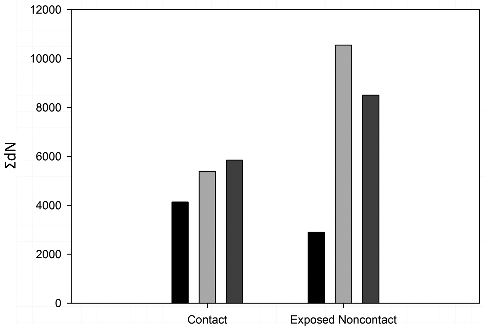
\includegraphics[width=0.8\textwidth]{Apendices/Publicaciones/Contact/Figures/figure4.pdf}
\caption{\small{Exposed noncontact residues from COX 1 are conspicuously conserved. Exposed noncontact residues from COX 1 are conspicuously conserved. The Contact and Exposed Noncontact sets from each mtDNA-encoded chain were used to compute the corresponding ${\Sigma}dN$ values. Black, light grey and dark grey bars represent COX 1, 2 and 3, respectively. From this figure, it is evident that exposed noncontact residues from COX 1 exhibit little tendency to mutate.}}
\label{paper34}
\end{figure}
%

From the comparison of ${\Sigma}dN$ between subunits, it becomes clear-cut that exposed noncontact residues from COX 1 are particularly constrained (Fig. \ref{paper34}). However, if we compare the inertia to changes of this subset of residues with respect to the rest of COX 1 resides, we may wonder whether exposed noncontact residues from COX 1 are significantly more conserved than the rest of COX 1 residues. To address this question while avoiding assumptions about the underlying distributions, we resorted to a bootstrap approach. Briefly, for each mtDNA-encoded chain, the codons from the multiple sequence alignment were randomly sorted to form a subset of the same size than the original Exposed Noncontact subset of the corresponding chain. Afterwards, ${\Sigma}dN$ was computed using this random subset. For each chain, the random resampling was performed 10$^{4}$ times to build up empirical distributions,
which were used to contrast the ${\Sigma}dN$ values computed in the real Exposed Noncontact subsets. As it can be deduced from Fig. \ref{paper35}, those residues belonging to the Exposed Noncontact groups from COX 2 and COX 3 are among the most variable residues (p-values 0.003 and 0.045, respectively). In contrast, exposed noncontact residues from COX 1 were among the most conserved residues (Fig. \ref{paper35}).

% Fig 5
\begin{figure}
\centering
\includegraphics[width=0.4\textwidth]{Apendices/Publicaciones/Contact/Figures/figure5.pdf}
\caption{\small{The behaviour of exposed noncontact residues from COX 1 diverges from that exhibited for their counterparts in COX 2 and COX 3. For each mtDNA-encoded chain the codons from the multiple sequence alignment were randomly sorted to form a subset of the same size than the original Exposed Noncontact subset of the corresponding chain. Afterwards, ${\Sigma}dN$  was computed using this random subset. For each chain, the random resampling was performed 10$^4$ times to build up empirical distributions, which were used to contrast the ${\Sigma}dN$ values computed in the real Exposed Noncontact subsets, which are indicated as filled circles on the abscissa axis.}}
\label{paper35}
\end{figure}
%

In an attempt to get further insight into the particular forces imposing such exceptionally high degree of conservation between exposed noncontact COX 1 residues, we assessed the effect of in silico alanine scanning mutagenesis on the stability of the complex. Although the mean ${\Delta}{\Delta}$G for exposed noncontact COX 1 residues (1.64 kJ/mol) was significantly higher than those values from COX 2 (1.20 kJ/mol) and COX 3 (1.16 kJ/mol), p- values 0.015 and 0.008, respectively, the contribution of COX 1 exposed noncontact residues to the whole thermodynamic stability of the holoenzyme can hardly be invoked as a reason for their high degree of conservation, as it is evident from Fig. \ref{paper36}. For each mtDNA-encoded protein, the Contact and Exposed Noncontact subsets were employed to compute their ${\Sigma}dN$ values, which were plotted against their corresponding ${\Delta}{\Delta}$G mean values (Fig. \ref{paper36}). We found a significant (p-value = 0.035) negative correlation between these two variables, indicating that those substitutions that tend to be more destabilizing are also more constrained, which is in line with our previous observations that thermodynamic stability plays a relevant role in the evolvability of mtDNA-encoded proteins (Aledo et al. 2012). However, the COX 1 Exposed Noncontact group showed up as an outlier. In this sense, for a ${\Delta}{\Delta}$G of 1.64 kJ/mol (the mean value computed for COX 1 exposed noncontact residues) the expected ${\Sigma}dN$ should be higher than twice the observed ${\Sigma}dN$ (Fig 6). In other words, whatever the constraining forces may be, they seem to be unrelated to structural stability.

% Fig 6
\begin{figure}
\centering
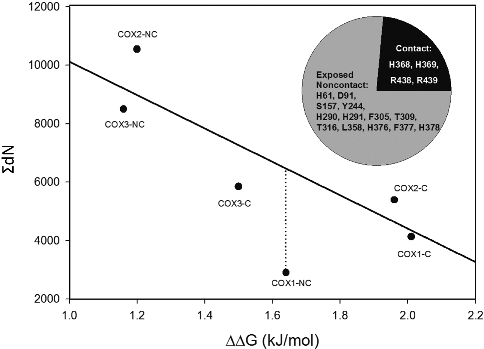
\includegraphics[width=0.6\textwidth]{Apendices/Publicaciones/Contact/Figures/figure6.pdf}
\caption{\small{Exposed noncontact residues from COX 1 are much more conserved than expected from their destabilizing effect on the holoenzyme. The exposed residues from each mtDNA-encoded proteins were split into two groups: contact (C) and noncontact (NC), according to the criteria given in the text. Afterwards, the ${\Sigma}dN$ and mean ${\Delta}{\Delta}$G were computed for each of these subsets. These two variables showed a significant negative correlation (n = 6, Pearson r = -0.774, p-value = 0.035) that was improved when data corresponding to COX 1 Exposed Noncontact were excluded from the analysis (n=5, Pearson r = -0.890, p-value = 0.021). The inset shows the proportion of residues that have been described as functionally relevant present among the Exposed Noncontact (grey), in comparison with the proportion of these residues that belong to the Contact group (black).}}
\label{paper36}
\end{figure}
%

Thus, we next explored other alternatives. In this sense, it is widely acknowledged that functional regions of proteins exhibit higher inertia to nonsynonymous changes than those other regions (Glaser et al. 2003). Hence, if there were a higher proportion of functionally important residues in the exposed noncontact region of COX 1 than in its contact counterpart, this would help to explain the extraordinarily low ${\Sigma}dN$ computed for the set Exposed Noncontact from COX 1. To test this possibility, we focused on those COX 1 residues that have been described to fulfil important functions such as the binding of heme, Cu and Mg, proton pumping and electron transfer (Michel et al. 1998; Yoshikawa 1998). Figure \ref{paper36} inset shows that the proportion of these residues that belong to the Exposed Noncontact set override the proportion of those that pertain to the Contact group. Although this observation is qualitatively in line with the very low ${\Sigma}dN$ observed for the COX 1 Exposed Noncontact ensemble, it should be noted that the catalogue of COX 1 functional residues we have used, is very limited in size and probably it is far from the complete inventory, which hampers obtaining quantitative statistical support. Nevertheless, the exceptionally high degree of conservation observed between exposed noncontact COX 1 residues, likely captures important constraints that apply to biological functionality yet to be unravelled.

In this regard, we wondered whether this set of COX 1 exposed noncontact residues might be involved in functions related to the formation of mitochondrial supercomplexes. Indeed, during the past decade, significant experimental evidence supports the organization of the mitochondrial respiratory chain into higher order structures known as respirasome (Sch�gger and Pfeiffer 2000; Ac�n-P�rez et al. 2008; Winge 2012). Along the same lines, two quasi-simultaneous recent studies have reported the 3D structure of mitochondrial supercomplex I$_1$III$_2$IV$_1$, determined by electron cryo-microscopy at 19-22$\AA$ resolution (Althoff et al. 2011; Dudkina et al. 2011). Fitting of X-ray structures of single complexes I, III2 and IV with high fidelity, unravels only a few sites where neighbouring complexes come close enough for ion bridges or hydrogen bonds. Three of such sites of potentially strong protein-protein interaction were found between complexes III and IV. However, none of these sites were on COX 1 (Althoff et al. 2011; Dudkina et al. 2011). Nevertheless, beside the supercomplex I$_1$III$_2$IV$_1$, other forms of supercomplexes such as I$_1$III$_2$IV$_2$, I$_1$III$_2$IV$_3$ and I$_1$III$_2$IV$_4$, have been described in bovine heart mitochondria (Sch�gger and Pfeiffer 2001). Since the three dimensional structures of these less abundant forms of supercomplexes are unknown, the involvement of residues from COX 1 in the assembly/stability of respirasomes, although unlikely, cannot be completely ruled out. In any event, the high degree of conservation between the exposed noncontact residues from COX 1 herein described, is an unexpected and intriguing observation that we are currently unable to explain. Nevertheless, we have noted that when this particular behaviour of COX 1 noncontact residues is not properly accounted, it leads to high interaction ratios that may be misinterpreted as an optimizing high evolvability of Mt-nu contact residues.

\subsection*{Contact residues from nDNA-encoded proteins tend to be more constrained than their noncontact counterparts.}

A number of works have previously addressed the evolution of nDNA-encoded COX subunits (Schmidt et al. 2001; Das et al. 2004; Uddin et al. 2008; Osada and Akashi 2011). However, some of the conclusions drawn from these studies are in apparent conflict. For instance, Schmidt and coworkers concluded that while contact nDNA-encoded residues are subjected to a strong purifying selection (Schmidt et al. 2001), Osada and Akashi reached the conclusion that nDNA-encoded residues exhibit signs of positive selection (Osada and Akashi 2011). These conflicting results may be attributable to methodological differences. Thus, while the former authors assembled and analysed a data set formed by contact and noncontact residues without distinguishing between different COX subunits, the latter authors looked for individual sites under positive selection using the methodology described somewhere else (Zhang 2005). Herein, we have readdressed the issue employing a meso approach, consisting in analysing each individual nDNA-encoded chain.

As a first approach, we computed the interaction ratio for each subunit. Contact residues tend to be more conserved than their noncontact counterpart, as suggested by R$_{1,2}$ values well below the unit, with the exception of COX 5A (Fig. \ref{paper37}A). This subunit is much more conserved than any of the other nuclear-encoded subunits (Fig. \ref{paper37}B). The high level of conservation, which extends beyond the contact residues, suggests that subunit 5A has been subjected to an exceptionally strong purifying selection. Supporting this implication of functional constraint is experimental evidence for ligand interaction that involves subunit COX 5A as a receptor of 3,5-diiodothyronine, able to abolish the allosteric inhibition of respiration by ATP (Arnold et al. 1998).

% Fig 7
\begin{figure}
\centering
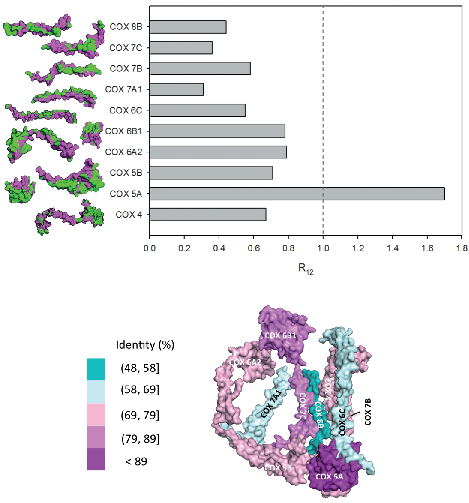
\includegraphics[width=0.7\textwidth]{Apendices/Publicaciones/Contact/Figures/figure7.pdf}
\caption{\small{COX 5A, a highly conserved protein, is the only nDNA-encoded subunit with an
interaction ratio R$_{1,2}$ higher than the unit. (A) For each nDNA-encoded COX subunit, the
${\Sigma}dN$ value for the Contact and Noncontact sets were computed to calculate the interaction ratio
$R_{1,2}$. As it can be deduced from this figure, contact residues (magenta) tend to be more conserved than their noncontact counterpart (green), with the only exception of COX 5A. (B) To gain an indication of the relative rates of change among nuclearly encoded subunits, an alignment data set was constructed using only those species for which all the nDNA-encoded subunits were represented (\textit{Ailuropoda melanoleuca}, \textit{Bos taurus}, \textit{Cavia porcellus}, \textit{Equus caballus}, \textit{Mus musculus}, \textit{Rattus norvegicus} and \textit{Sus scrofa}). Using this data set, the percentage of identity was computed for each subunit. Again COX 5A stood up, in this case as an exceptionally conserved protein.}}
\label{paper37}
\end{figure}
%

In general lines, the results summarized in Fig. \ref{paper37}A are consistent with those obtained by other authors using the pooled sequences (Schmidt et al. 2001). In analysing each individual nDNA-encoded polypeptide, we aimed to detect those subunits that might exhibit a particular evolutionary behaviour. However, such goal faced methodological challenges. Probably, the most important methodological limitation was the impossibility, because of the small size of the nDNA-encoded COX subunits, of obtaining a statistically relevant sample of residues. Therefore, in the absence of a large enough sample of residues, the herein computed R$_{1,2}$ values can only give a qualitative indication of the trend, but they lack of statistical significance. To overcome such inconvenience, we resorted to nonparametric analyses.

For a given subunit, each residue was labeled as 'variant' or 'invariant', depending on its conservation throughout a multisequence alignment (Supplementary Material-2). On the other hand, according to the criterion already described, the same residue was classified as 'contact' or 'exposed noncontact'. In this way, the proportion of variant exposed noncontact residues ($p_0$) and that of variant contact residues ($p_1$) were computed, as well as its differences, $d = p_0 - p_1$. According to a null hypothesis where the variability of a residue is independent of its role in intersubunit interaction, these differences should fit to a symmetric distribution with zero median. To test such a hypothesis, a Wilcoxon signed-rank test was carried out, resulting in the rejection of the null hypothesis (p $<$ 0.007). Thus, the higher proportion of variable residues among the exposed noncontact positions with respect to the contact positions (see Table from Supplementary Material-3) are unlikely to be due to chance.

\section*{Concluding remarks}
Interactions of mtDNA- and nDNA-encoded proteins provide unique opportunities to study the evolution of protein-protein interactions and the effects of these interactions on the evolution of their respective genomes. To this respect, mammalian COX complex is well suited for studying the evolution of within- and between-genome interactions because a functional complex requires three mtDNA-encoded and ten nDNA-encoded subunits, accounting for a large number of interacting residues. Previous studies carried out with this complex, have suggested that mtDNA-encoded residues in close physical contact with nDNA- encoded amino acids may be subjected to positive selection to optimize the structural- functional interaction between subunits from different genetic origins. This conclusion was based on the higher rate of nonsynonymous substitutions observed among mtDNA-encoded residues in contact with nDNA-encoded residues, with respect to the rest of mtDNA-encoded amino acids. However, as we have shown herein, failing to discern the effect of interaction from other confounding factors such as the solvent exposure, can lead to misleading conclusions. Thus, when such corrections were made, data analysis showed that mtDNA- encoded residues engaged in contacts are, in general, more constrained than their noncontact counterparts. Nevertheless, noncontact residues from the surface of COX 1 subunit are a remarkable exception, being subjected to an exceptionally high purifying selection.

Besides providing compelling evidence against the so-called optimizing interaction hypothesis, our approach also allowed to make some interesting findings. For instance, those mtDNA-encoded residues in contact with mtDNA-encoded residues from a different chain, are subjected to stronger constrains than those involved in interactions with nDNA-encoded subunits. This observation cannot be explained on the basis of thermodynamic stability, because interactions between mtDNA-encoded subunits contribute more weakly to the complex stability than those interactions between subunits encoded by different genomes. Therefore, the higher conservation observed among mtDNA-encoded residues involved in within genome interactions, is likely due to functional rather than structural reasons.

\section*{Material and Methods}
\subsection*{DNA Sequences}
A collection of 371 mammalian mitochondrial genomes was obtained from the National Center for Biotechnology Information (NCBI) genome database (\url{www.ncbi.nlm. nih.gov}). For the analyses involving COX subunits encoded by nuclear genes, sequences from a variable number of species ranging from 14 to 30 (depending on sequence availability) were acquired from NCBI. A complete list of the mammalian taxa used and the accession number of the sequences is provided as Supplementary Material-4. Orthologous sequences were aligned by codons using ClustalW (the alignments can be retrieved from \url{http://mecom.hval.es}).

\subsection*{Codon sorting}
Using the sequence from Bos taurus as reference and the crystal structure of bovine COX (Protein Data Bank, PDB, 2OCC), each codon position from the above described alignments, was sorted into different subsets according to the algorithm sketched in Figure \ref{paper31}. Briefly, the data set corresponding to all the codons from the alignment of a given COX subunit (for instance, chain A, corresponding to COX 1, which is a mtDNA-encoded subunit), was initially divided into two subsets: Contact and Noncontact, depending on whether the encoded amino acid from chain A, is or not closer than 4$\AA$ to a residue from any polypeptide other than chain A, respectively. Interacting positions were defined as being $<$ 4$\AA$ apart because this is the upper limit for weak interactions (Martin et al. 1997). Afterwards, the Contact set was, in turn, split into two subsets: Intergenomic Contact (Mt-nu Contact, in the example) and Intragenomic Contact (Mt-mt Contact, in the example). The criterion to assign a given codon into the former subset was that the interacting residues should be encoded by different genomes, otherwise the codon is allocated into the latter subset. On the other hand, the Noncontact set was split up into two subsets: Exposed Noncontact and Buried Noncontact, on the basis of solvent accessible surface areas of the considered residue (Aledo et al. 2012). Computation of physical distances between residues and the sorting procedure was assisted by an \emph{ad hoc} computer program that we have called MECOM (Molecular Evolution of protein COMplexes), which, together with the corresponding manual, can be downloaded from \url{http://mecom.hval.es}.

\subsection*{Nonsynonymous sequence divergences and statistics}
Nonsynonymous sequence divergences were calculated from pairwise comparisons using the alignment data subsets described in the precedent section and employing the method of maximum likelihood implemented in PAML 4.6 (Yang and Nielsen 2000; Yang 2007). The sum of these nonsynonymous sequence divergences for all the pairwise comparisons was computed and denoted as ${\Sigma}dN_i$, where the subscript, $i$, refers to the subset used for the calculations (Fig. \ref{paper31}).

Since we aimed to test for statistical evidence of the existence of differential
evolutionary patterns among residues belonging to different subsets, we used the so-called
interaction ratio (Schmidt et al. 2001), $R$, defined as the ratio between the ${\Sigma}dN$ for the sets $i$ being tested. For instance, if we want to compare residues involved in intersubunit contacts (subset 1) with the rest of residues, which are not implicated in such interactions (subset 2), we compute $R_{1,2} = {\Sigma}dN_1 / {\Sigma}dN_2$. In this way, a $R_{1,2}$ value indistinguishable from 1 should be interpreted as that both set of residues show similar nonsynonymous substitution rates. $R_{1,2}$ $<$ 1 would result from a reduced evolutionary rate among the residues belonging to subset 1, relative to those residues from subset 2. On the contrary, $R_{1,2}$ $>$ 1 points to a higher rate of nonsynonymous substitutions among residues from subset 1, with respect to those belonging to subset 2. To determine when $R_{i,j}$ differs from 1 because of a differential pattern of evolution and when it may be due to statistical uncertainty, a Z-test was performed to assess the significance of these deviations.

For mtDNA-encoded subunits (chains A, B and C corresponding to COX1, COX2 and COX3, respectively), which are the larger subunits from complex IV (514, 227 and 261 residues, respectively), it was possible to generate a reliable random distribution of ${\Sigma}dN_i$. To this end, the codons from multiple sequence alignments of each chain were randomly sorted into two subsets of the same sizes than the original subset $i$. Afterwards, ${\Sigma}dN_i$ was computed as explained above. The random resampling was performed 10$^4$ times to build up an empirical distribution.

In order to calculate the number of nonsynonymous substitutions per nonsynonymous site on a lineage-by-lineage basis, we used a maximum likelihood method (F3x4 model) implemented in codeml from the PAML package (Yang 2007). To this end, the phylogenetic tree of seven mammalian species (\textit{Bos taurus}, \textit{Sus scrofa}, \textit{Equus caballus}, \textit{Ailuropoda melanoleuca}, \textit{Mus musculus}, \textit{Rattus norvegicus} and \textit{Cavia porcellus}) for which the gene sequences of the 13 COX subunits were available, was reconstructed using \textit{Arbacia lixula} as an outgroup. This tree and the alignments corresponding to the different residue categories were used to apportion the nonsynonymous substitutions among lineages.

\subsection*{Relative evolutionary rate}
The codon alignment for each subunit was subjected to MEGA5 (Tamura et al. 2011) to calculate the relative evolutionary rate, RER. This software implements a maximum likelihood method and makes use of the Jones-Taylor-Thornton substitution model (Jones et al. 1992) to estimate the relative evolutionary rate at each single site. A discrete Gamma (+G) distribution was used to model evolutionary rate differences among sites. Five discrete Gamma categories were considered. The computed rates were scaled such that the average evolutionary rate across all sites is 1. This means that sites showing a rate lower than 1 are evolving slower than average, and those with a rate higher than 1 are evolving faster than average.

\subsection*{Thermodynamic stability changes}
The thermodynamic stability changes, ${\Delta}{\Delta}$G, of mutations were computed using the protein design tool FoldX version 3.0 (Guerois et al. 2002; Schymkowitz et al. 2005). FoldX uses a full atomic description of the structure of the protein, to provide a quantitative estimation of the importance of the interactions contributing to the stability of this protein. The 3D structure of COX was subjected to an optimization procedure using the repair function of FoldX. Afterwards, an alanine scan was carried out, the resulting ${\Delta}{\Delta}$G were recorded and used to calculate the means for Exposed Noncontact, Mt-mt Contact and Mt-nu Contact residues.

\section*{Acknowledgments}
This work was supported by grant CGL2010-18124 from the Ministerio de Ciencia e Innovaci�n, Spain. We thank Alicia Esteban del Valle and Miguel �ngel Medina for their helpful comments on the manuscript.

\section*{References}
\begin{itemize}
\item[]{Ac�n-P�rez R, Fern�ndez-Silva P, Peleato ML, P�rez-Martos A, Enr�quez JA. 2008. Respiratory Active Mitochondrial Supercomplexes. \textit{Mol Cell} 32:529-539.}
\item[]{Alba MM, Catresana J. 2005. Inverse Relationship Between Evolutionary Rate and Age of Mammalian Genes. \textit{Mol Biol Evol} 22:598-606.}
\item[]{Aledo JC. 2004. Glutamine breakdown in rapidly dividing cells: waste or investment? \textit{Bioessays} 26:778-785.}
\item[]{Aledo JC, Li Y, de Magalh�es JP, Ru�z-Camacho M, P�rez-Claros JA. 2010. Mitochondrially encoded methionine is inversely related to longevity in mammals. \textit{Aging Cell} 10:198- 207.}
\item[]{Aledo JC, Valverde H, Ru�z-Camacho M. 2012. Thermodynamic Stability Explains the Differential Evolutionary Dynamics of Cytochrome b and COX I in Mammals. \textit{J Mol Evol} 74:69-80.}
\item[]{Althoff T, Mills DJ, Popot J-L, K�hlbrandt W. 2011. Arrangement of electron transport chain components in bovine mitochondrial supercomplex I1III2IV1. \textit{EMBO J} 30:4652-4664.}
\item[]{Arnold S, Goglia F, Kadenbach B. 1998. 3,5-Diiodothyronine binds to subunit Va of cytochrome-c oxidase and abolishes the allosteric inhibition of respiration by ATP. \textit{Eur J Biochem} 252:325-330.}
\item[]{Azevedo L, Carneiro J, van Asch B, Moleirinho A, Pereira F, Amorim A. 2009. Epistatic interactions modulate the evolution of mammalian mitochondrial respiratory complex components. \textit{BMC Genomics} 10:266.}
\item[]{Barrientos A, M�ller S, Dey R, Wienberg J, Morales CT (2000) Cytochrome c oxidase assembly in primates is sensitive to small evolutionary variations in amino acid sequence. \textit{Mol. Biol. Evol.} 17, 1508-1519.}
\item[]{Castellana S, Vicario S, Saccone C. 2011. Evolutionary Patterns of the Mitochondrial Genome in Metazoa: Exploring the Role of Mutation and Selection in Mitochondrial Protein-Coding Genes. \textit{Genome Biol Evol} 3:1067-1079.}
\item[]{Castresana J, L�bben M, Sarste M, Higgins DG. 1994. Evolution of cytochrome oxidase, an enyme older than atmospheric oxygen. \textit{EMBO J} 13:2516-2525.}
\item[]{Das J, Miller ST, Stern DL. 2004. Comparison of Diverse Protein Sequences of the Nuclear- Encoded Subunits of Cytochrome C Oxidase Suggests Conservation of Structure Underlies Evolving Functional Sites. \textit{Mol Biol Evol} 21:1572-1582.}
\item[]{Dudkina NV, Kudryashev M, Stahlberg H, Boekema EJ. 2011. Interaction of complexes I, III, and IV within the bovine respirasome by single particle cryoelectron tomography. \textit{Proc. Natl Acad Sci USA} 108:15196-15200.}
\item[]{Edmands S \& Burton RS. 1999. Cytochrom c oxidase activity in interpopulation hybrids of a marine copepod: a test for nuclear-nuclear or nuclear-cytoplasmic coadaptation. \textit{Evolution} 53:1972-1978.}
\item[]{Glaser F, Pupko T, Paz I, Bell RE, Bechor-Shental D, Martz E, Ben-Tal N. 2003. ConSurf: Identification of functional regions in proteins by surface-Mapping of phylogenetic information. \textit{Bioinformatics} 19:163-164.}
\item[]{Guerois R, Nielsen JE \& Serrano L. 2002. Predicting Changes in the Stability of Proteins and Protein Complexes: A Study of More Than 1000 Mutations. \textit{J Mol Biol} 320:369-387.}
\item[]{Jones DT, Taylor WR, Thornton JM. 1992. The rapid generation of mutation data matrices from protein sequences. \textit{Computer Applications in the Biosciences} 8:275-282.}
\item[]{Kenyon L, Moraes CT. 1997. Expanding the functional human mitochondrial DNA database by the establishment of primate xenomitochondrial cybrids. \textit{Proc Natl Acad Sci USA} 94:9131-9135.}
\item[]{Little AG, Kocha KM, Lougheed SC, Moyes CD. 2010. Evolution of the nuclear-encoded cytochrome oxidase subunits in vertebrates. \textit{Physiological Genomics} 42:76-84.}
\item[]{de Magalh�es JP. 2005. Human Disease-Associated Mitochondrial Mutations Fixed in Nonhuman Primates. \textit{J Mol Evol} 61:491-497.}
\item[]{Martin PD, Michael GM, Box J, Esmon CT, Edwards BF. 1997. New insights into the regulation of the blood clotting cascade derived from the X-ray crystal structure of bovine meizothrombine des F1 in complex with PPACK. \textit{Structure} 5:1681-1693.}
\item[]{McKenzie M. 2003. Functional Respiratory Chain Analyses in Murid Xenomitochondrial Cybrids Expose Coevolutionary Constraints of Cytochrome b and Nuclear Subunits of Complex III. \textit{Mol Biol Evol} 20:1117-1124.}
\item[]{Michel H, Behr J, Harrenga A, Kannt A. 1998. Cytochrome c Oxidase: Structure and Spectroscopy. \textit{Annu Rev Biophys Biomol Struct} 27:329-356.}
\item[]{Osada N, Akashi H. 2011. Mitochondrial-Nuclear Interactions and Accelerated Compensatory Evolution: Evidence from the Primate Cytochrome c Oxidase Complex. \textit{Mol Biol Evol} 29:337-346.}
\item[]{Sch�gger H, Pfeiffer K. 2000. Supercomplexes in the respiratory chains of yeast and mammalian mitochondria. \textit{EMBO J} 19:1777-1783.}
\item[]{Sch�gger H, Pfeiffer K. 2001. The ratio of oxidative phosphorylation complexes I-V in bovine heart mitochondria and the composition of respiratory chain supercomplexes. \textit{J Biol Chem} 276:37861-37867.}
\item[]{Schmidt TR, Wildman DE, Uddin M, Opazo JC, Goodman M \& Grossman LI. 2005. Rapid electrostatic evolution at the binding site for cytochrome c on cytochrome c oxidase in anthropoid primates. \textit{Proc Natl Acad Sci USA} 102:6379-6384.}
\item[]{Schmidt TR, Wu W, Goodman M, Grossman LI. 2001. Evolution of nuclear- and mitochondrial-encoded subunit interaction in cytochrome c oxidase. \textit{Molecular Biology and Evolution} 18:563-569.}
\item[]{Schymkowitz J, Borg J, Stricher F, Nys R, Rousseau F \& Serrano L. 2005. The FoldX web server: an online force field. \textit{Nucleic Acids Research} 33:W382-W388.}
\item[]{Soto IC, Fontanesi F, Liu J \& Barrientos A. 2012. Biogenesis and assembly of eukaryotic cytochrome c oxidase catalytic core. \textit{Biochimica et Biophysica Acta (BBA) - Bioenergetics} 1817:883-897.}
\item[]{Suen DF, Norris KL, Youle RJ. 2008. Mitochondrial dynamics and apoptosis. \textit{Genes \& Development} 22:1577-1590.}
\item[]{Tamura K, Peterson D, Peterson N, Stecher G, Nei M, Kumar S. 2011. MEGA5: Molecular Evolutionary Genetics Analysis Using Maximum Likelihood, Evolutionary Distance, and Maximum Parsimony Methods. \textit{Mol Biol Evol} 28:2731-2739.}
\item[]{Uddin M, Opazo JC, Wildman DE, Sherwood CC, Hof PR, Goodman M, Grossman LI. 2008. Molecular evolution of the cytochrome c oxidase subunit 5A gene in primates. \textit{BMC Evol Biol} 8:8.}
\item[]{Vishnoi A, Kryazhimskiy S, Bazykin GA, Hannenhalli S, Plotkin JB. 2010. Young proteins experience more variable selection pressures than old proteins. \textit{Genome Res} 20:1574-1581.}
\item[]{Willett CS. 2003. Evolution of Interacting Proteins in the Mitochondrial Electron Transport System in a Marine Copepod. \textit{Mol Biol Evol} 21:443-453.}
\item[]{Winge DR. 2012. Sealing the Mitochondrial Respirasome. \textit{Mol Cell Biol} 32:2647-2652.} 
\item[]{Yang Z. 2007. PAML 4: Phylogenetic Analysis by Maximum Likelihood. \textit{Mol Biol Evol} 24:
1586-1591.}
\item[]{Yang Z, Nielsen R. 2000. Estimating synonymous and nonsynonymous substitution rates
under realistic evolutionary models. \textit{Mol Biol Evol} 17:32-43.}
\item[]{Yoshikawa S. 1998. Redox-Coupled Crystal Structural Changes in Bovine Heart Cytochrome
c Oxidase. \textit{Science} 280:1723-1729.}
\item[]{Zhang J. 2005. Evaluation of an Improved Branch-Site Likelihood Method for Detecting
Positive Selection at the Molecular Level. \textit{Mol Biol Evol} 22:2472-2479.}
\end{itemize}
